% Manuscript v3 | 2026-09-27 | BDG selected; final comparative results pending.
% Build from paper/: pdflatex main; bibtex main; pdflatex main; pdflatex main.
% Previous live sources and PDF: versions/v2_pre_v3_2026-09-27/.
\documentclass{article}
\PassOptionsToPackage{numbers,compress}{natbib}
\usepackage[final,main]{neurips_2026}
\usepackage[utf8]{inputenc}
\usepackage[T1]{fontenc}
\usepackage{amsmath,amssymb,booktabs,graphicx,microtype,url}
\usepackage{algorithm,algpseudocode}
\usepackage{xcolor,tikz}
\usetikzlibrary{arrows.meta,positioning}
\usepackage{hyperref}
\hypersetup{hidelinks,pdftitle={BDG: Batch-Dispersion Guidance for Property-Band Generation},pdfsubject={Manuscript v3, 27 September 2026}}
\newcommand{\pend}{\textcolor{black!60}{\textsf{P}}}
\newcommand{\Fbar}{\bar F}
\newcommand{\Vb}{V_b}
\newcommand{\weff}{w_{\mathrm{eff}}}
\newcommand{\IB}{\mathrm{IB}}
\newcommand{\sg}{\operatorname{stopgrad}}
\title{BDG: Batch-Dispersion Guidance for\\Property-Band Generation}
\author{Bobo Li, Henry Huang, Idea Idehpour, Haimo Fang\\
Department of Computer and Information Science, University of Pennsylvania\\
\small Manuscript v3 \quad 27 September 2026}
\begin{document}
% MAIN_TEXT_START
\maketitle
\begin{abstract}
Property-targeted generation requires samples to fall within a tolerance band while retaining sample quality and diversity. A single guidance strength scales both the displacement toward the target and the contraction of predicted properties within a batch. We introduce Batch-Dispersion Guidance (BDG), an inference-time rule that adjusts the deviation coefficient using the difference between the batch variance of predicted endpoint properties and a specified variance. BDG preserves the target-centering coefficient and uses the same network evaluations as plug-in guidance, with additional batch reductions. We study the rule on QM9 molecular coordinates and DeepFlyBrain DNA sequences represented on a probability simplex. The molecular study includes a matched comparison of linear flow matching and variance-preserving diffusion, a guided-versus-unguided comparison, and ablations of the dispersion gain and setpoint. Flow matching is the current development backbone; its empirical selection remains contingent on the base-model comparison. The sequence implementation retains the scalar feedback rule and changes the generator, property map, and state constraints. Algebraically, BDG reweights the plug-in direction through a batch-dependent gain and effective target, which defines the scope of the proposed contribution. Final comparative results are pending, so improvements in band coverage, sample quality, and transfer remain unresolved. The study tests whether feedback on property dispersion provides a useful quality--control trade-off beyond ordinary guidance-strength adjustment.
\end{abstract}

\section{Introduction}
Diffusion reverses a corruption process, and flow matching learns transport along a prescribed probability path \citep{karras2022elucidating,lipman2022flow}. We compare their suitability for controlled molecular generation.

Gradient guidance steers a frozen generator toward a target \citep{chung2023dps,song2023lgd}. Its quadratic property energy couples target centering and contraction, motivating a separate dispersion coefficient. Ensemble interactions and moment constraints already appear in prior work \citep{corso2024particle,mgd2026moment}; the question here is whether feedback from a learned endpoint property improves the quality--control trade-off.

We introduce BDG and study it on QM9 coordinates and DeepFlyBrain DNA simplices. We compare linear FM and VP diffusion, test plug-in guidance, ablate BDG, and plan recent-method benchmarks. We hypothesize that adjusting dispersion separately from target centering improves band coverage at comparable sample quality, with the same rule applicable to both state spaces. Our contributions are summarized as follows.
\begin{itemize}
\item We specify a paired molecular evaluation of the base models and guidance rules.
\item We define BDG and derive its relation to plug-in guidance and its widening condition.
\item We specify controls for dispersion gain, setpoint, strength, and feedback.
\item We implement the same scalar rule for sequences and specify how to assess transfer.
\end{itemize}

\section{Related Work}
\textbf{Continuous generation.} Flow matching fits conditional path velocities \citep{lipman2022flow}; diffusion design choices affect sampling quality and cost \citep{karras2022elucidating}. Our comparison holds the molecular representation and network size fixed and reports actual training and sampling budgets.

\textbf{Batch-dependent guidance.} Particle Guidance couples samples through a joint potential \citep{corso2024particle}. Moment Guided Diffusion targets prescribed moments \citep{mgd2026moment}, and Variance-Tilted Diffusion favors spread in a fixed linear feature space \citep{vtd2026variance}. BDG uses the residual between the empirical variance of endpoint property predictions and a user-set variance. Its contribution is this feedback rule within an existing guidance direction; batch coupling and moment targeting have prior precedent.

\textbf{Molecular comparisons.} Equivariant diffusion and EquiFM generate 3D molecules \citep{hoogeboom2022equivariant,song2023equifm}. DPS-style plug-in, LGD-MC, TMPD-inspired guidance, and TFG provide gradient, Monte Carlo, moment-based, and training-free alternatives on a frozen generator \citep{chung2023dps,song2023lgd,boys2024tmpd,ye2024tfg}. Appendix~\ref{app:comparisons} discloses their adaptations.

\textbf{Sequence comparisons.} Dirichlet FM uses simplex paths, Fisher Flow uses categorical information geometry, and MOG-DFM guides biological sequence design \citep{stark2024dirichlet,davis2024fisher,chen2025multi}. These are the three planned external sequence comparators. Their biological scores require a common protocol before comparison with our property-band task.

\section{Methods}
\subsection{Modalities, Data, and Preprocessing}\label{sec:data}
QM9 \citep{ramakrishnan2014qm9} contains 133{,}885 molecules in our DeepChem packaging. Coordinates are centered, and H/C/N/O/F types use unscaled one-hot features. The generator and guide $f_A$ use 51{,}527 training molecules; evaluator $f_B$ uses a disjoint 51{,}527. Validation and test contain 17{,}748 and 13{,}083 molecules. Targets are dipole moment $\mu$ (D), polarizability $\alpha$ (Bohr$^3$), and HOMO--LUMO gap (Ha).

DeepFlyBrain \citep{stark2024dirichlet} contains 500-base-pair enhancer sequences, embedded as A/C/G/T one-hot vectors on $(\Delta^3)^{500}$ and decoded by positionwise $\arg\max$. Retained train/validation/test counts are 83{,}722/10{,}505/10{,}434 after excluding four ambiguous training sequences. The generator is unconditional. This simplex state differs from Euclidean coordinates and their rotation symmetry (Appendix~\ref{app:data}).

\subsection{Continuous Flow Matching Baseline}\label{sec:fm}
For data $x_1$, Gaussian source $x_0$, and $t\sim\mathcal U(0,1)$, the path and loss are
\begin{equation}
x_t=t x_1+(1-t)x_0,\qquad
\mathcal L_{\mathrm{FM}}=\mathbb E\|v_\theta(x_t,t)-(x_1-x_0)\|_M^2.
\label{eq:fm}
\end{equation}
The masked norm separately averages coordinate and type errors with equal weight. Coordinate noise has zero center of mass. Our E(3)-equivariant EGNN has width 256, eight layers, and 3.75\,M parameters. The configuration uses Adam, learning rate $2\times10^{-4}$ with cosine decay, batch 256, 1{,}500 epochs, and EMA 0.9999. Sampling uses 100 Euler steps (Appendix~\ref{app:training}).

\subsection{Diffusion Baseline}\label{sec:diff}
The matched VP implementation uses the same representation, split, network size, and configured training budget. With noising time $u:0\to1$ and projected Gaussian noise $\epsilon$,
\begin{equation}
\begin{aligned}
x_u&=a(u)x_1+\sigma(u)\epsilon,\quad a(u)=e^{-\frac12(0.1u+9.95u^2)},\quad \sigma^2=1-a^2,\\
\mathcal L_{\mathrm{VP}}&=\mathbb E\|\epsilon_\phi(x_u,u)-\epsilon\|_M^2.
\end{aligned}
\label{eq:vp}
\end{equation}
The probability-flow ODE is $\mathrm dx/\mathrm du=-\tfrac12\beta(u)(x+s_\phi)$, where $\beta(u)=0.1+19.9u$ and $s_\phi=-\epsilon_\phi/\sigma$. A decreasing 100-step grid and terminal denoising use 101 network evaluations. External EDM is a separate comparison.

\subsection{Guided Generation}\label{sec:guidance}
For target $y$ and scale $s=f_A.\texttt{y\_std}>0$, plug-in guidance uses energy $(f_A(m_i)-y)^2/(2s^2)$. The endpoint estimate is $m_i=x_t^{(i)}+(1-t)v_\theta(x_t^{(i)},t)$. Define $F_i=f_A(m_i)$ and $J_i=\partial m_i/\partial x_t^{(i)}$. The field and clipped correction are
\begin{equation}
G_i=\frac{y-F_i}{s^2}J_i^\top\nabla_m f_A(m_i),\qquad
C_i=\operatorname{clip}_{\|v_i\|}\!\left(w\frac{1-t}{t}G_i\right).
\label{eq:plug}
\end{equation}
Here $\operatorname{clip}_r$ limits the correction norm to $r$; Euler advances with $v_i+C_i$. Guidance operates for $t\ge0.5$. The generator and guide are frozen; $f_B$ is used only for evaluation.

\subsection{Proposed Innovation: Batch-Dispersion Guidance}\label{sec:bdg}
BDG tests whether adjusting dispersion independently at the coefficient level improves band coverage. For $B\ge2$, define $\Fbar=B^{-1}\sum_iF_i$, $\Vb=(B-1)^{-1}\sum_i(F_i-\Fbar)^2$, and $\tau=\tau_{\mathrm{mult}}s>0$. Replace $y-F_i$ in Equation~\eqref{eq:plug} with
\begin{equation}
n_i=(y-F_i)-\eta e(F_i-\Fbar)=(y-\Fbar)-\weff(F_i-\Fbar),\qquad
e=\frac{\Vb-\tau^2}{\tau^2},\quad \weff=1+\eta e.
\label{eq:bdg}
\end{equation}
The gain $\eta\ge0$ changes the deviation coefficient; the centering coefficient remains one before the shared scale $w$. This does not imply independent control of realized mean and variance after the Jacobian and clipping.

Positive $e$ strengthens contraction. Negative $e$ weakens it; net repulsion requires $\weff<0$, or $\eta>1$ and $\Vb<\tau^2(1-1/\eta)$. For $\weff\ne0$, $n_i=\weff(y_{\mathrm{eff}}-F_i)$ with $y_{\mathrm{eff}}=(y+\eta e\Fbar)/\weff$. At $\weff=0$, Equation~\eqref{eq:bdg} remains finite. BDG retains the plug-in direction with a state-dependent gain and target. No setpoint-convergence guarantee follows.

Coefficients are held fixed during the vector--Jacobian product (Algorithm~\ref{alg:bdg}). BDG adds batch reductions, with no extra neural evaluations relative to plug-in. The $\eta=0$ ablation recovers plug-in. The one-sided variant uses $\max(e,0)$ and recovers plug-in only when its added term vanishes. Gain/setpoint and strength sweeps test separate effects; replay and signed-strength controls address the need for feedback.

\subsection{Transfer to Modality 2}\label{sec:transfer}
The sequence model uses a linear path from a Dirichlet$(1,1,1,1)$ source and a dilated one-dimensional CNN. BDG retains Equation~\eqref{eq:bdg}; soft GC fraction and CpG frequency replace the learned guide. Euler steps are clamped and renormalized onto the simplex, then decoded for exact counts. Projection enforces feasibility; the scalar rule alone does not ensure a tangent update. Timing and batch settings remain unresolved (Appendix~\ref{app:m2}).

\subsection{Model Overview}\label{sec:overview}
Figure~\ref{fig:overview} connects the molecular comparison to the transferred controller.
\begin{figure}[htbp]
\centering
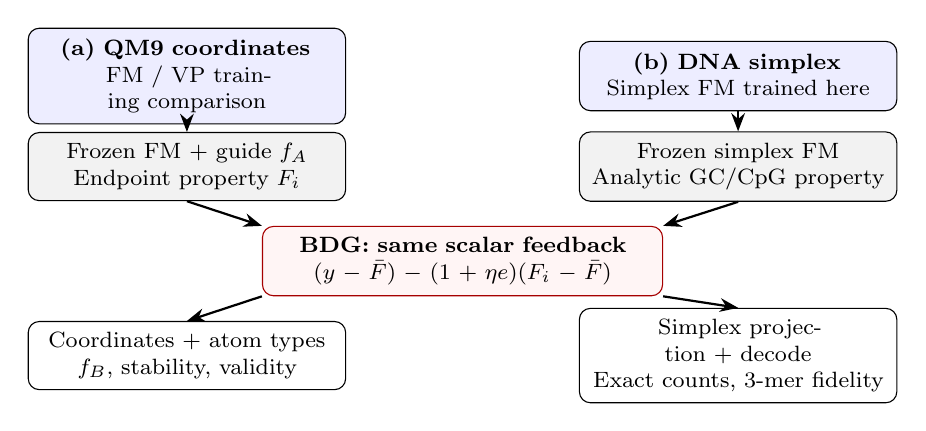
\begin{tikzpicture}[font=\footnotesize,box/.style={draw,rounded corners,align=center,inner sep=4pt,text width=3.75cm},arr/.style={-{Stealth},thick}]
\node[box,fill=blue!7] (m1) at (0,0) {\textbf{(a) QM9 coordinates}\\FM / VP training comparison};
\node[box,fill=blue!7] (m2) at (7,0) {\textbf{(b) DNA simplex}\\Simplex FM trained here};
\node[box,fill=black!5] (g1) at (0,-1.15) {Frozen FM + guide $f_A$\\Endpoint property $F_i$};
\node[box,fill=black!5] (g2) at (7,-1.15) {Frozen simplex FM\\Analytic GC/CpG property};
\node[box,draw=red!65!black,fill=red!4,text width=4.8cm] (b) at (3.5,-2.35) {\textbf{BDG: same scalar feedback}\\$(y-\bar F)-(1+\eta e)(F_i-\bar F)$};
\node[box] (o1) at (0,-3.55) {Coordinates + atom types\\$f_B$, stability, validity};
\node[box] (o2) at (7,-3.55) {Simplex projection + decode\\Exact counts, 3-mer fidelity};
\draw[arr] (m1)--(g1); \draw[arr] (m2)--(g2);
\draw[arr] (g1.south)--(b.north west); \draw[arr] (g2.south)--(b.north east);
\draw[arr] (b.south west)--(o1.north); \draw[arr] (b.south east)--(o2.north);
\end{tikzpicture}
\caption{Two-modality study. Blue identifies project model development; gray identifies frozen sampling components; red marks BDG's shared rule. Backbone selection awaits matched FM--VP results. External checkpoints enter separate comparisons.}
\label{fig:overview}
\end{figure}

\section{Results}
\subsection{Evaluation Protocol}\label{sec:protocol}
Final measurements are pending; \pend{} denotes an unavailable result in Tables~\ref{tab:fmvd}--\ref{tab:m2}. QM9 band coverage is $\IB=n^{-1}\sum_i\mathbf1\{|f_B(\hat x_i)-y|\le\delta\}$ on decoded samples, with median training target $y$ and $\delta=2\operatorname{MAE}_{\mathrm{cal}}(f_B)$. We will report it beside molecule stability, RDKit validity, uniqueness, and distinct-valid yield per attempt. Predicted spread is distinct from molecular diversity.

The molecular protocol fixes $w=1$, batch $B=500$, and three paired sampling seeds. The operator chooses $n$, divisible by 500. Arms share initial noise, atom counts, checkpoints, targets, and evaluator within each backend. We will report seed means, standard deviations, and paired differences. BDG couples samples within a batch, so molecule-level independence is insufficient for uncertainty estimates. All arms remain visible; no chemistry threshold excludes a result. Equal $w$ denotes equal nominal strength, not equal force (Appendix~\ref{app:evaluation}).

\subsection{Modality 1: Flow Matching versus Diffusion}\label{sec:fmvd}
The matched comparison (Table~\ref{tab:fmvd}) will test whether quality and cost support the development backbone. External EDM results cannot replace the comparison between the models trained here.

\begin{table}[!htbp]
\centering\small
\caption{Matched QM9 base models. Metrics are seed mean $\pm$ seed standard deviation; results and runtime are pending. NFE includes terminal denoising. Quality metrics are fractions.}
\label{tab:fmvd}
\begin{tabular}{lccccc}
\toprule
Model & Mol. stab.$\uparrow$ & Validity$\uparrow$ & Uniqueness$\uparrow$ & NFE$\downarrow$ & Time$\downarrow$\\
\midrule
FM, trained here & \pend & \pend & \pend & 100 & \pend\\
VP, trained here & \pend & \pend & \pend & 101 & \pend\\
\bottomrule
\end{tabular}
\end{table}


\subsection{Modality 1: Guided versus Unguided Generation}\label{sec:guidworks}
The paired comparison will test target improvement and chemistry cost (Table~\ref{tab:guidance}). A final guidance benefit remains unresolved.

\begin{table}[!htbp]
\centering\small
\caption{QM9 guidance at $w=1$, separately for $\mu$, $\alpha$, and gap. IB is band coverage; DV is distinct-valid molecules per attempt. All results are pending.}
\label{tab:guidance}
\begin{tabular}{lccccc}
\toprule
Arm & IB$\uparrow$ & Mol. stab.$\uparrow$ & Validity$\uparrow$ & Uniqueness$\uparrow$ & DV$\uparrow$\\
\midrule
Unguided & \pend & \pend & \pend & \pend & \pend\\
Plug-in & \pend & \pend & \pend & \pend & \pend\\
\bottomrule
\end{tabular}
\end{table}


\subsection{Modality 1: Innovation Ablations}\label{sec:ablations}
The registered grid uses $\eta\in\{1,2,4,8\}$, $\tau_{\mathrm{mult}}\in\{0.5,0.75,1,1.5\}$, and one $\eta=0$ setting, at $w\in\{1,4\}$. Seeds, $n$, and $B$ match the headline run. Table~\ref{tab:ablation} identifies the controls. Clipping frequency and realized gain must accompany attribution to dispersion.

\begin{table}[!htbp]
\centering\small
\caption{BDG controls. The first two rows belong to the registered grid; additional controls have no final results. $\Delta$IB is the paired change from plug-in; $R$ is decoded property standard deviation divided by unguided.}
\label{tab:ablation}
\begin{tabular}{llccc}
\toprule
Control & Effect isolated & $\Delta$IB & $R$ & Mol. stab.$\uparrow$\\
\midrule
$\eta=0$ & identity to plug-in & \pend & \pend & \pend\\
Gain/setpoint, $w=1,4$ & dispersion vs. strength & \pend & \pend & \pend\\
One-sided residual & negative-residual branch & \pend & \pend & \pend\\
Open-loop replay & feedback vs. schedule & \pend & \pend & \pend\\
Signed-strength plug-in & scalar reweighting & \pend & \pend & \pend\\
\bottomrule
\end{tabular}
\end{table}


\subsection{Modality 1: Comparison with Recent Methods}\label{sec:recent}
Table~\ref{tab:recent} reserves four recent guidance comparisons per flow backend. Results stay within backend because property pairs and acceptance widths differ. Cost includes generator/gradient passes, runtime, and memory.

\begin{table}[!htbp]
\centering\small
\caption{Molecular guidance at $w=1$, per property and backend. BDG uses $\eta=4$, $\tau_{\mathrm{mult}}=0.5,1.0$, reported separately. Prior-method rows are adaptations. Results are pending.}
\label{tab:recent}
\begin{tabular}{lcccc}
\toprule
Method & IB$\uparrow$ & Mol. stab.$\uparrow$ & DV$\uparrow$ & Time$\downarrow$\\
\midrule
DPS-style plug-in \citep{chung2023dps} & \pend & \pend & \pend & \pend\\
TMPD-inspired \citep{boys2024tmpd} & \pend & \pend & \pend & \pend\\
LGD-MC \citep{song2023lgd} & \pend & \pend & \pend & \pend\\
TFG \citep{ye2024tfg} & \pend & \pend & \pend & \pend\\
BDG (ours) & \pend & \pend & \pend & \pend\\
\bottomrule
\end{tabular}
\end{table}


\subsection{Modality 2: Transfer of the Innovation}\label{sec:m2}
Sequence evaluation will pair exact GC/CpG band coverage with 3-mer Jensen--Shannon divergence and sequence diversity (Table~\ref{tab:m2}). Implementation alone does not establish empirical transfer. Protocol alignment and measurements remain pending.

\begin{table}[!htbp]
\centering\small
\caption{Planned DeepFlyBrain comparisons at length 500, separately by property. JSD measures 3-mer mismatch; diversity is mean normalized pairwise Hamming distance. All comparisons remain pending.}
\label{tab:m2}
\begin{tabular}{lcccc}
\toprule
Method & IB$\uparrow$ & JSD$\downarrow$ & Diversity$\uparrow$ & Time$\downarrow$\\
\midrule
Simplex FM, unguided & \pend & \pend & \pend & \pend\\
Simplex FM + plug-in & \pend & \pend & \pend & \pend\\
Simplex FM + BDG & \pend & \pend & \pend & \pend\\
Dirichlet FM \citep{stark2024dirichlet} & \pend & \pend & \pend & \pend\\
Fisher Flow \citep{davis2024fisher} & \pend & \pend & \pend & \pend\\
MOG-DFM \citep{chen2025multi} & \pend & \pend & \pend & \pend\\
\bottomrule
\end{tabular}
\end{table}


\subsection{Cross-Modality Analysis and Failure Modes}\label{sec:failure}
Transfer will be assessed through within-modality changes from plug-in. Predictor error can separate guided and evaluated molecular properties; sequence relaxation and decoding can create a similar mismatch with exact counts. Clipping and simplex projection can distort the correction. Diagnostics are needed before attributing gains or failures to BDG.

\section{Discussion}
BDG adds a dispersion residual to the guidance coefficient. Its algebra separates target centering from deviation weighting and identifies when the latter becomes repulsive. The common gradient direction limits the contribution to an adaptive coefficient rule.

Final measurements must determine whether BDG improves coverage at comparable quality, survives strength and feedback controls, and transfers to DNA. A spread change alone would support a narrower mechanism claim. Pending model selection, predictor reliability, batch dependence, and unmatched external evaluation limit stronger conclusions.
% MAIN_TEXT_END
\clearpage
\bibliographystyle{ieeetr}
\bibliography{citation,refs_extra}
\clearpage
\appendix
\section{Reproducibility and Extended Protocol}
\subsection{Data Sources and Splits}\label{app:data}
The QM9 source is the DeepChem/MoleculeNet packaging. The project retains the 3{,}054 entries removed as uncharacterized in common EDM preprocessing, so its data definition differs from those benchmarks. A seeded permutation creates the splits. Centering removes translation; predictors are invariant. Coordinates and one-hot types have no additional scaling. Predictors use training-derived property normalization. Molecular sizes are paired across arms within each backend.

DeepFlyBrain is stored in \path{proj1/m2/blade_bundle/dfb500.npz}. Four ambiguous training examples were excluded from the supplied 83{,}726. The channel order is A/C/G/T and length is 500. Cell-type labels are not supplied to our unconditional generator. Random-example splits do not establish sequence-cluster or out-of-distribution generalization. The older 200-base-pair Kenyon-cell setup is excluded from the final comparison.

\subsection{Training and Checkpoint Records}\label{app:training}
Table~\ref{tab:training} separates configurations from final provenance. Matching configurations does not establish equal completed training. Checkpoints, actual epochs, and selection rules must accompany FM--VP evaluation. The existing FM record uses final EMA weights; VP code selects by validation generation stability with loss as tie-breaker. This difference must be disclosed or aligned before selection.

\begin{table}[!htbp]
\centering\small
\caption{Training configuration and recorded properties. Asterisks mark configured settings requiring final run verification. P denotes missing final provenance. Predictor counts are per property network.}
\label{tab:training}
\begin{tabular}{llll}
\toprule
Setting & Molecular FM / VP & $f_A$ / $f_B$ & Sequence FM\\
\midrule
Architecture & EGNN, 256, 8 layers & invariant EGNN, 128, 4 & CNN, 128, 10 layers\\
Parameters & 3.75 M each & 429{,}825 each & approximately 1.02 M\\
Training split & \texttt{train\_a} & \texttt{train\_a} / \texttt{train\_b} & DeepFlyBrain train\\
Objective & velocity / noise MSE & property MSE & velocity MSE\\
Epochs & 1{,}500$^*$ & 120 & 1{,}500 recorded\\
Batch & 256$^*$ & 128 & 256\\
Optimizer & Adam$^*$ & Adam & \pend\\
Learning rate & $2\times10^{-4}$, cosine$^*$ & $3\times10^{-4}$, cosine & $2\times10^{-3}$, cosine\\
EMA & 0.9999$^*$ & none & \pend\\
Run seed & 20260918$^*$ & \pend & \pend\\
Hashes / hardware & \pend & \pend & \pend\\
\bottomrule
\end{tabular}
\end{table}

For coordinates $c$ and features $f$, the norm in Equations~\eqref{eq:fm} and~\eqref{eq:vp} is
\[
\|z\|_M^2=\frac{\|M\odot z^c\|_2^2}{3\sum M}+\frac{\|M\odot z^f\|_2^2}{5\sum M}.
\]
The mask $M$ broadcasts over channels. Coordinate noise is projected to zero center of mass, giving dimension $3(N-1)$ for $N$ atoms. Feature noise is Gaussian. Atom types use the largest final feature component. VP time $u$ is clean-to-noise; flow time $t$ is noise-to-data.

\subsection{Evaluation and Cost Accounting}\label{app:evaluation}
The molecular protocol fixes seeds 20261001, 20261002, and 20261003, q50 targets, $w=1$, $t_{\min}=0.5$, and batch 500. Per-cell $n$ is operator-selected and divisible by 500. Each cell runs $n/500$ separately coupled batches. Increasing $n$ adds batches without changing each variance estimator's sample count. Batch size is a BDG design parameter.

The calibration pool contains 3{,}000 molecules from the two training halves. Internal predictors are calibrated only on the half they did not train on. Evaluator-specific acceptance widths differ from $\tau=\tau_{\mathrm{mult}}f_A.\texttt{y\_std}$. Final cells record widths and predictor identities (Table~\ref{tab:backends}).

\begin{table}[!htbp]
\centering\small
\caption{Molecular guidance backends. External generators are pretrained and frozen. Results stay within backend. External EDM is separate from our trained VP comparison.}
\label{tab:backends}
\begin{tabular}{lll}
\toprule
Generator & Guide / evaluator & Headline arms\\
\midrule
Our FM & internal disjoint pair & all seven\\
External EquiFM & released TFG pair & all seven\\
External EDMsecond & internal disjoint pair & unguided, plug-in\\
\bottomrule
\end{tabular}
\end{table}

The seven arms are unguided, plug-in, TMPD-inspired, LGD-MC, TFG, and BDG at $\eta=4$, $\tau_{\mathrm{mult}}\in\{0.5,1\}$. Two setpoints cannot establish a monotone curve; the ablation supplies additional gains and setpoints. All arms remain visible regardless of stability. The pilot chemistry floor does not govern this protocol.

Atom stability is the fraction satisfying the project's bond/valence rules; molecule stability requires all atoms to pass. RDKit validity uses fixed reconstruction and sanitization. Uniqueness divides distinct canonical SMILES by valid samples; distinct-valid yield divides distinct valid molecules by all attempts. We will report attempted, decoded, valid, and distinct-valid counts. Band coverage includes chemically invalid samples and cannot alone measure usable yield.

We distinguish $f_A$ endpoint spread as a controller diagnostic from $f_B$ decoded spread as an evaluation diagnostic. Neither equals structural diversity. The analysis will report three seed values, mean, sample standard deviation, and paired changes under common noise. Intervals must respect coupled batches. Sampling seeds quantify sampling variation at fixed weights, not training-seed uncertainty.

Cost accounting will include generator forwards, generator vector--Jacobian products, guide forwards/backwards, peak memory, and seconds per sample on matched hardware. BDG adds reductions to plug-in's calls; equal calls do not establish equal runtime. Final manifests will supply Monte Carlo counts and optimization steps.

\subsection{Baseline Adaptations and Comparison Limits}\label{app:comparisons}
Our DPS-style plug-in adapts inverse-problem guidance to a Gaussian property energy and flow endpoint. TMPD-inspired guidance linearizes property uncertainty. LGD-MC and TFG also require disclosed endpoint, noise, and sampler choices. These adaptations do not reproduce every published benchmark.

External EquiFM and EDMsecond differ from our FM--VP pair in data, architecture, and parameterization. EquiFM uses TFG predictors with different acceptance widths and uncertain training overlap. Coverage comparisons stay within backend and predictor pair.

Dirichlet FM, Fisher Flow, and MOG-DFM require common length, target, band width, conditioning, decoding, and reference data. Published class-conditioned scores do not establish GC/CpG-band performance. These rows are pending evaluations. Guidance ports on our sequence generator do not themselves reproduce these three models.

\subsection{Sequence Transfer Protocol}\label{app:m2}
The shipped model is \path{proj1/m2/blade_bundle/fm_m2_dfb500.pt}. Its path joins a uniform Dirichlet source to one-hot sequences. The sampler clamps each Euler update to nonnegative values, renormalizes per position, and decodes by $\arg\max$. Endpoint extrapolation used by the guide need not lie on the simplex, creating a possible mismatch with decoded counts.

For relaxed sequence $p\in\mathbb R^{L\times4}$,
\[
F_{\mathrm{GC}}(p)=L^{-1}\sum_{j=1}^L(p_{j,C}+p_{j,G}),\qquad
F_{\mathrm{CpG}}(p)=(L-1)^{-1}\sum_{j=1}^{L-1}p_{j,C}p_{j+1,G}.
\]
GC is affine; CpG is quadratic. Evaluation counts bases or adjacent pairs after decoding. Exact counts have no prediction error to define a nonzero band. Existing code uses $\delta=\max(0.16s,4.4/(L-1))$, with training-property standard deviation $s$. GC/CpG counting increments are $1/L$ and $1/(L-1)$; the current floor uses the latter for both. Final widths must be fixed before comparison and are not commensurate with molecular bands.

Final sequence timing, batch size, $n$, seeds, and comparator alignment remain unspecified. The driver defaults to $t_{\min}=0$; earlier pilots used $0.5$. Table~\ref{tab:m2} requires one declared protocol.

Three-mer JSD compares generated and held-out frequencies. Diversity is mean normalized pairwise Hamming distance, with the pair-sampling rule recorded. Evaluation will also include decoding confidence and duplicates. Composition statistics do not establish enhancer activity or cell-type specificity.

\subsection{BDG Algorithm and Algebraic Limits}
Algorithm~\ref{alg:bdg} gives the update. All weights are fixed. Batch statistics determine coefficients; the pullback differentiates properties with coefficients held fixed. Differentiating a loss through the coefficients would produce another update.

\begin{algorithm}[htbp]
\caption{One BDG-guided Euler step}\label{alg:bdg}
\begin{algorithmic}[1]
\Require batch $x_t$, frozen $v_\theta$ and $f$, target $y$, scale $s>0$, gain $\eta\ge0$, setpoint $\tau>0$, strength $w$, step $h$, start $t_{\min}$
\State $v\gets v_\theta(x_t,t)$
\If{$t<t_{\min}$} \State \Return $\Pi(x_t+h v)$ \EndIf
\State $m\gets x_t+(1-t)v_\theta(x_t,t)$ with gradients enabled
\State $F_i\gets f(m_i)$; $\Fbar\gets B^{-1}\sum_iF_i$
\State $\Vb\gets (B-1)^{-1}\sum_i(F_i-\Fbar)^2$ if $B>1$, else $\tau^2$
\State $e\gets(\Vb-\tau^2)/\tau^2$ \Comment{one-sided: $e\gets\max(e,0)$}
\State $a_i\gets\sg\{[(y-F_i)-\eta e(F_i-\Fbar)]/s^2\}$
\State $G\gets\operatorname{VJP}_{x_t}(F,a)$
\State $C_i\gets w(1-t)/\max(t,\varepsilon)\,G_i$
\State $C_i\gets C_i\min(1,\|v_i\|/\max(\|C_i\|,\varepsilon))$
\State \Return $\Pi\{x_t+h(v+C)\}$
\end{algorithmic}
\end{algorithm}

For molecules, $\Pi$ applies masks and coordinate centering; for sequences it clamps and renormalizes. The numerical guard $\varepsilon$ is implementation-specific. The sequence score factor uses $10^{-6}$. At $B=1$, $F_i-\Fbar=0$ and dispersion vanishes even though the sequence code records a different variance fallback.

The bound $\weff\ge1-\eta$ follows from $\Vb\ge0$. In the simplified property ODE $\dot F_i=(y-\Fbar)-\weff(F_i-\Fbar)$, $\dot V_b=-2\weff V_b$. For $\eta>1$, a positive stationary variance is $\tau^2(1-1/\eta)$, below the setpoint. This assumes homogeneous unit response, continuous time, and no generator drift, clipping, or projection. It gives no convergence guarantee for the implemented sampler.

\clearpage
\subsection{Implementation Map and Pending Evidence}\label{app:implementation}
Table~\ref{tab:provenance} connects the paper to the repository. Archived pilots remain available. No pilot effect substitutes for a pending final experiment.

\begin{table}[!htbp]
\centering\small
\caption{Source and evidence map, relative to the repository root. Final output trees and run manifests are pending.}
\label{tab:provenance}
\begin{tabular}{ll}
\toprule
Component & Source or protocol\\
\midrule
Molecular BDG & \path{proj1/src/guidance.py}, \texttt{mode == "bdg"}\\
Integration & \path{proj1/src/sampling.py}\\
VP training & \path{proj1/scripts/train_diffusion.py}\\
Final molecular sweep & \path{proj1/scripts/transfer_sweep.py}\\
Headline protocol & \path{docs/protocol/FULL_RUN_V3_PROTOCOL.md}\\
Ablation protocol & \path{docs/protocol/ABLATION_V3_PROTOCOL.md}\\
Sequence implementation & \path{proj1/m2/m2_sweep.py}\\
Sequence protocol status & \path{docs/protocol/MODALITY2_V3_PLAN.md}\\
Algebraic checks & \path{proj1/tests/test_bdg.py}\\
\bottomrule
\end{tabular}
\end{table}

\textbf{Run identity.} Each final result requires a generator checkpoint hash,
guide and evaluator identities, dataset/split identifiers, target and band width,
sample count, batch size, seed, integrator, step count, guidance window, nominal
strength, and method-specific settings. BDG additionally requires its gain,
setpoint multiplier, one-sided flag, and any replay schedule. A common method
name is insufficient to identify a matched comparison.

\textbf{Evidence status.} Implementation and algebraic checks address whether the
specified update is computed. They do not establish a coverage improvement,
sample-quality advantage, or successful transfer. Final empirical evidence must
come from the declared comparison protocol with per-seed measurements. Older
pilot outputs remain separate because their targets, strengths, batch sizes, or
sample counts can differ.

\textbf{Reproducibility record.} The final release will pair each aggregate with
its underlying cell records and analysis configuration. Hardware, software
versions, wall-clock costs, and peak memory will accompany the neural-call
counts. Configuration changes and failed or excluded runs require explicit
records. These identifiers are pending and are not reconstructed from the
current draft's table structure.


\end{document}
